\chapter{Chapter 2. Data sets and pre-processing}

The data in this study are from the Time History of Events and Macroscale Interactions during Substorms-Acceleration, Reconnection, Turbulence and Electrodynamics of the Moon’s Interaction with the Sun (THEMIS-ARTEMIS) mission  and the Magnetospheric Multiscale (MMS) mission. The former mission is optimized for observing different regions of the magnetosphere and near-Earth solar wind. The five probes traverse near-Earth space in different regions and orbits according to the science phases. The latter also moves through the solar wind and magnetosheath. MMS measurements from the Fast Plasma Instrument (FPI) and Fluxgate Magnetometer (FGM) are used along with THEMIS Electrostatic Analyzers (ESA) and Fluxgate Magnetometer (FGM) measurements. THEMIS and MMS mission data is accessible through the PySPEDAS software (\url{https://github.com/spedas/pyspedas}). Figure \ref{fig:orbits-all} shows the location of the THEMIS and MMS probes for the selected time periods. The orange orbit lines display portions of the MMS orbits from 2015-2023 in both the solar wind and magnetosheath. The pink, red, green, and blue orbit lines show the THEMIS orbits in 2008, 2009, 2018, and 2022. The solid line and dashed line are the estimated bow shock and magnetopause boundaries \cite{SlavinHolzer:1984,Shue:1997}. %A significant portion (green and red lines) of the coordinated analysis data periods are hidden behind the orange MMS orbit lines; however, the orbit plots for the coordinated analysis periods can be found in the appendix.

\begin{figure}
    \centering
    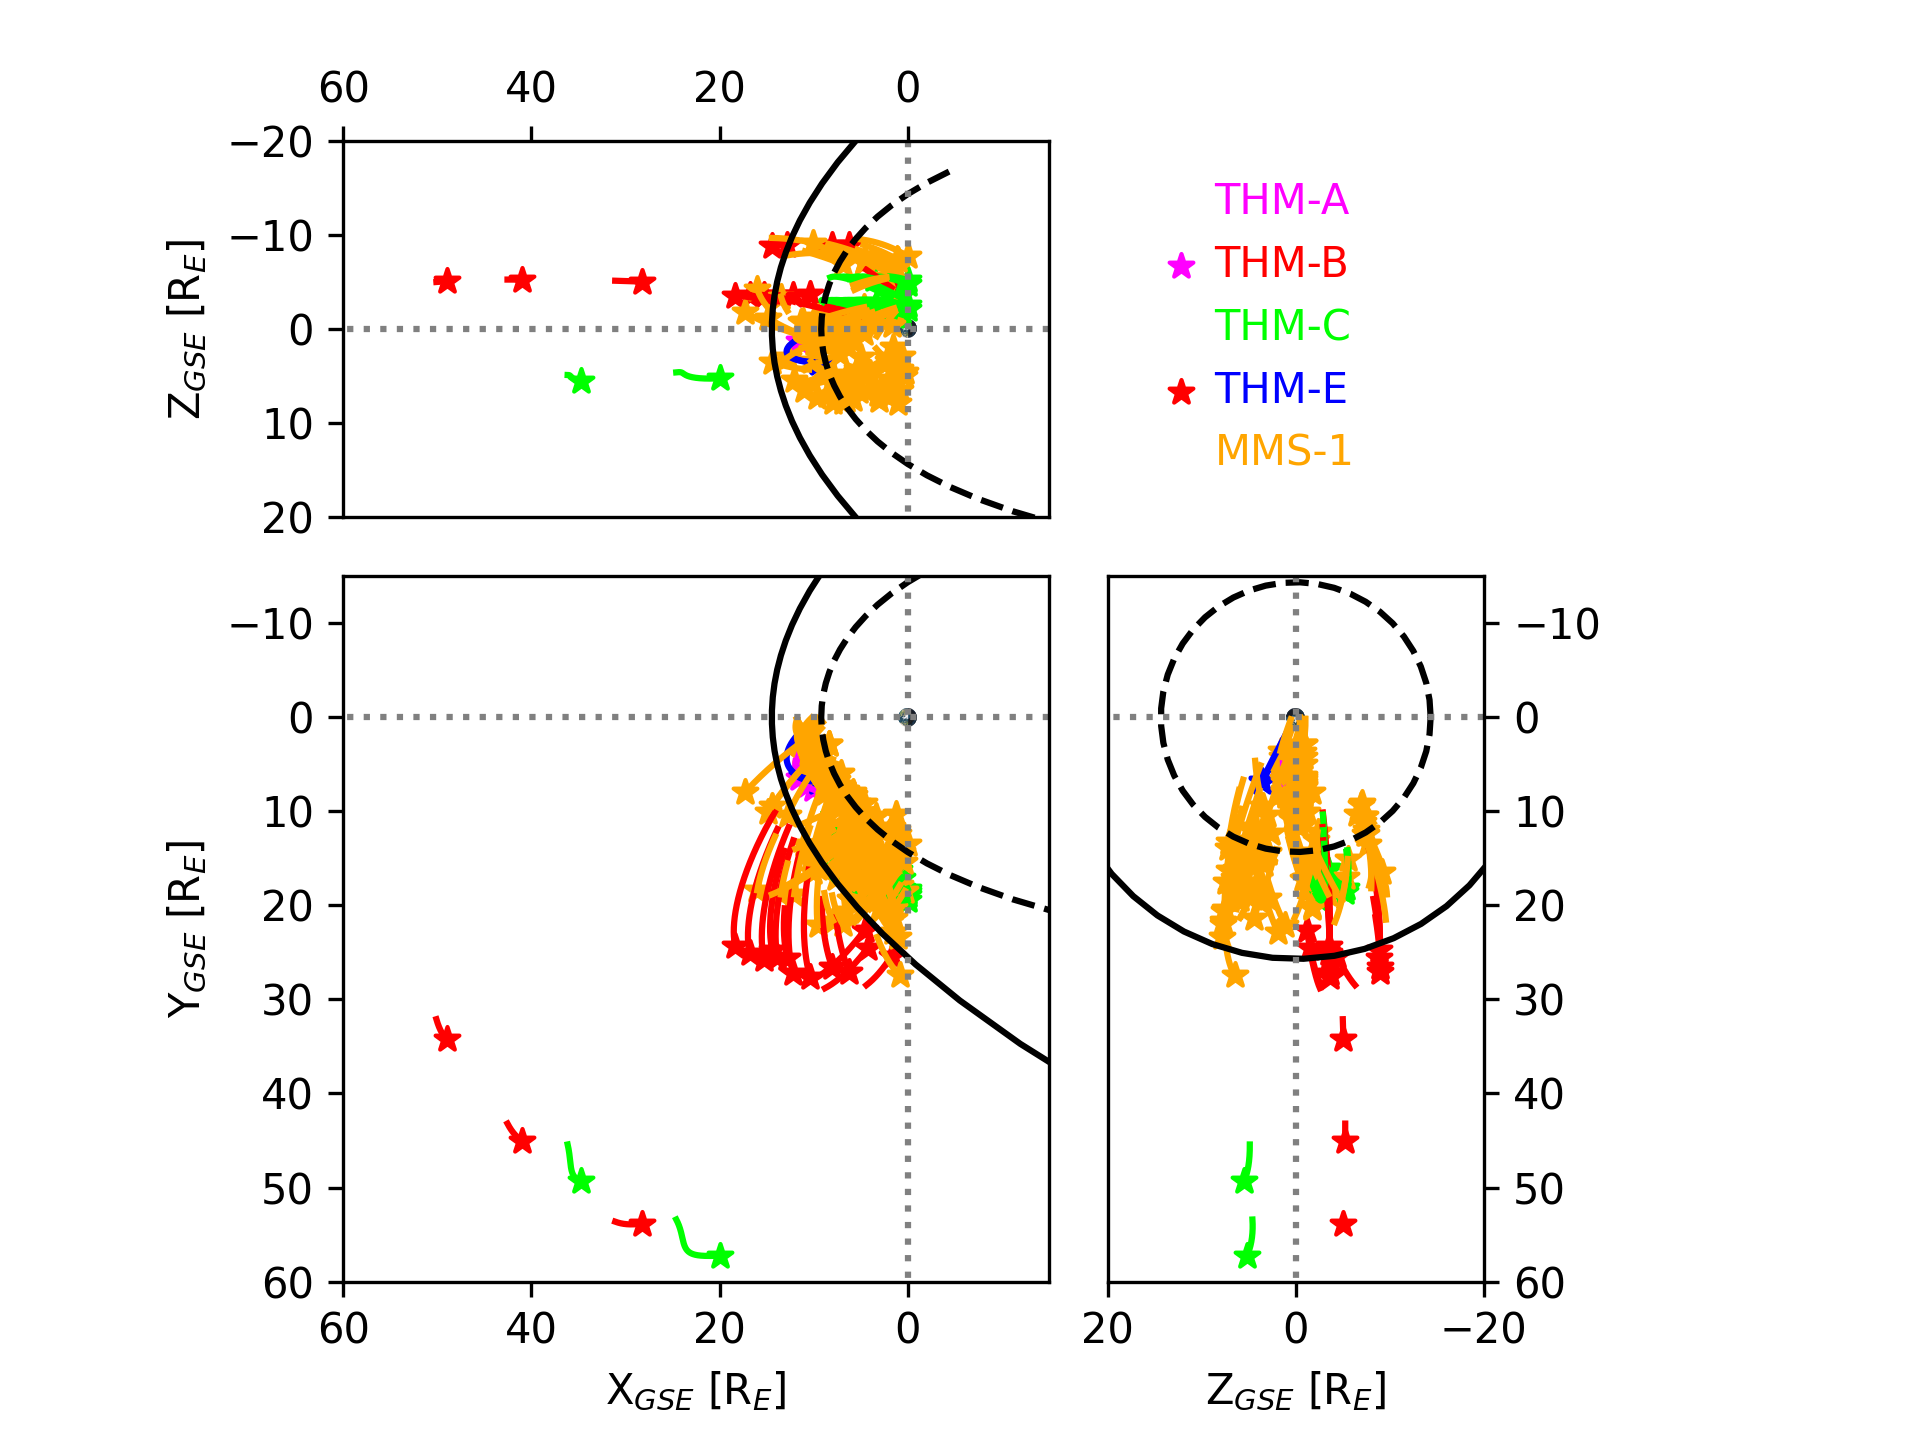
\includegraphics[width=\textwidth]{Figures/Orbits/all_TE_orbits_xy_xz_yz.png}
    \caption[Orbits for all observed time periods]{Orbits for all observed time periods, with the stars being the end of the orbit period. Magnetopause (dashed black line) modelled using the \cite{Shue:1997} model and bow shock (solid black line) modelled using \cite{SlavinHolzer:1984}. IMF data was obtained for one period in 2015, thus the boundaries are not accurate for all periods.}
    \label{fig:orbits-all}
\end{figure}

Hours-long periods of $\sim$3 second THEMIS and 4.5 second MMS data in the magnetosheath and near-Earth solar wind are chosen such that the search interval is entirely contained in one region to avoid transition regions. These time periods, ranging in lengths from approximately 6 hours to 26 hours, are identified by looking at time series data and simultaneous changes in magnetic field, density, velocity, and ion spectra. Short instances of bow shock crossings are identified in certain time periods, and the events identified in the crossing periods are removed from the final lists. Figure \ref{fig:timeseries-MMS-magnetosheath} and \ref{fig:timeseries-THM-magnetosheath} are an example of two observed time periods in the magnetosheath from MMS-1 and THM-C, respectively. Both figures show the time series of magnetic field, velocity, proton density, temperature, and ion energy spectra, as well as calculated values such as Alfv\'en velocity and plasma beta. These quantities are used in our analysis, as well as to identify the region in which spacecraft was located.

\begin{figure}
    \centering
    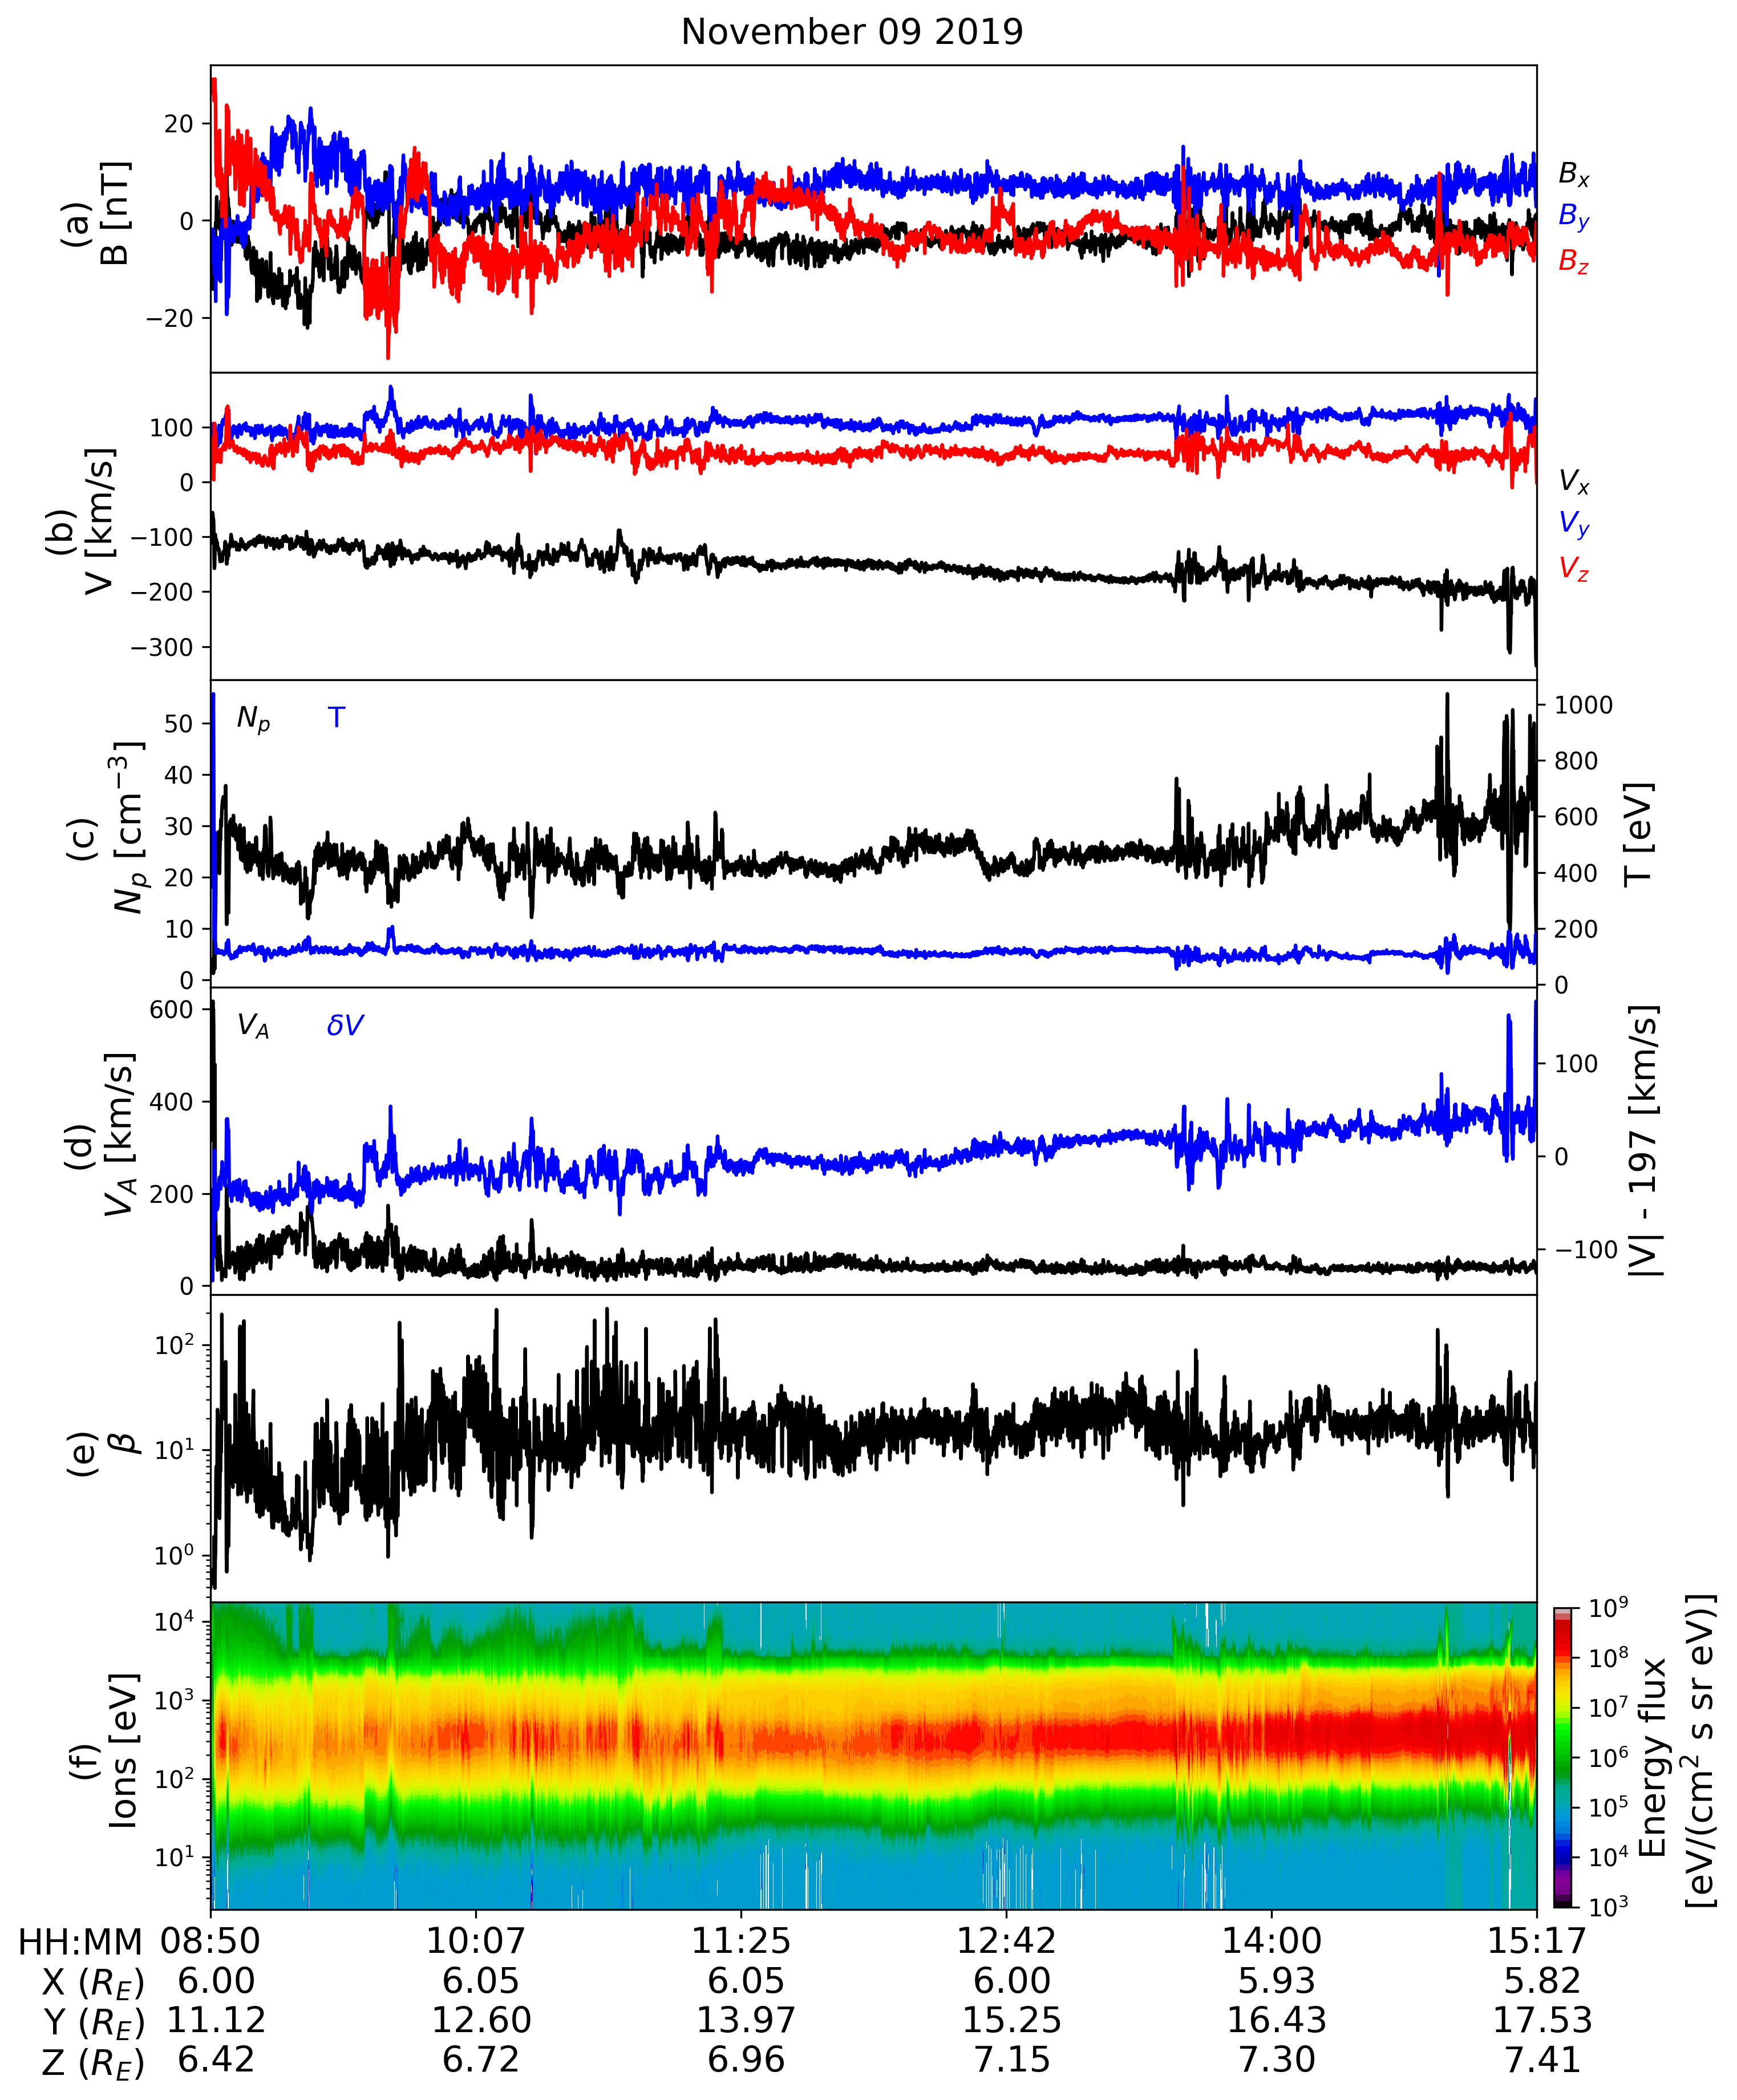
\includegraphics[width=\textwidth]{Figures/Time series/timeseries_09112019_MMS1.png}
    \caption[Time series data for MMS-1 on 9 November 2019]{a) magnetic field, b) velocity, c) density and temperature, d) Alfv\'en speed and fluctuations of the magnitude of the velocity, e) plasma beta, and f) ion spectra observed by MMS-1 for $\sim$6 hours in the magnetosheath on 9 November 2019.}
    \label{fig:timeseries-MMS-magnetosheath}
\end{figure}

% Coordinated study
The dayside science and radiation belt science phases of the THEMIS mission offer optimal configuration for direct comparison of the near-Earth solar wind and magnetosphere, specifically those in 2008, 2009, 2018, and 2022. MMS is also used in conjunction with the THEMIS probes for the time periods identified in 2022. 19 time intervals were identified during these phases for which there were simultaneous measurements by two THEMIS probes, where one was in the solar wind and one was in the magnetosheath. For the 2022 orbit phase, MMS-1 data was included for its respective region. It should be noted that the data came from simultaneous measurement in two regions during the same interval, \textit{not} a measurement across the bow shock. An orbit plot for just the coordinated study is shown in Figure \ref{fig:orbits-coordinated}.

\begin{figure}
    \centering
    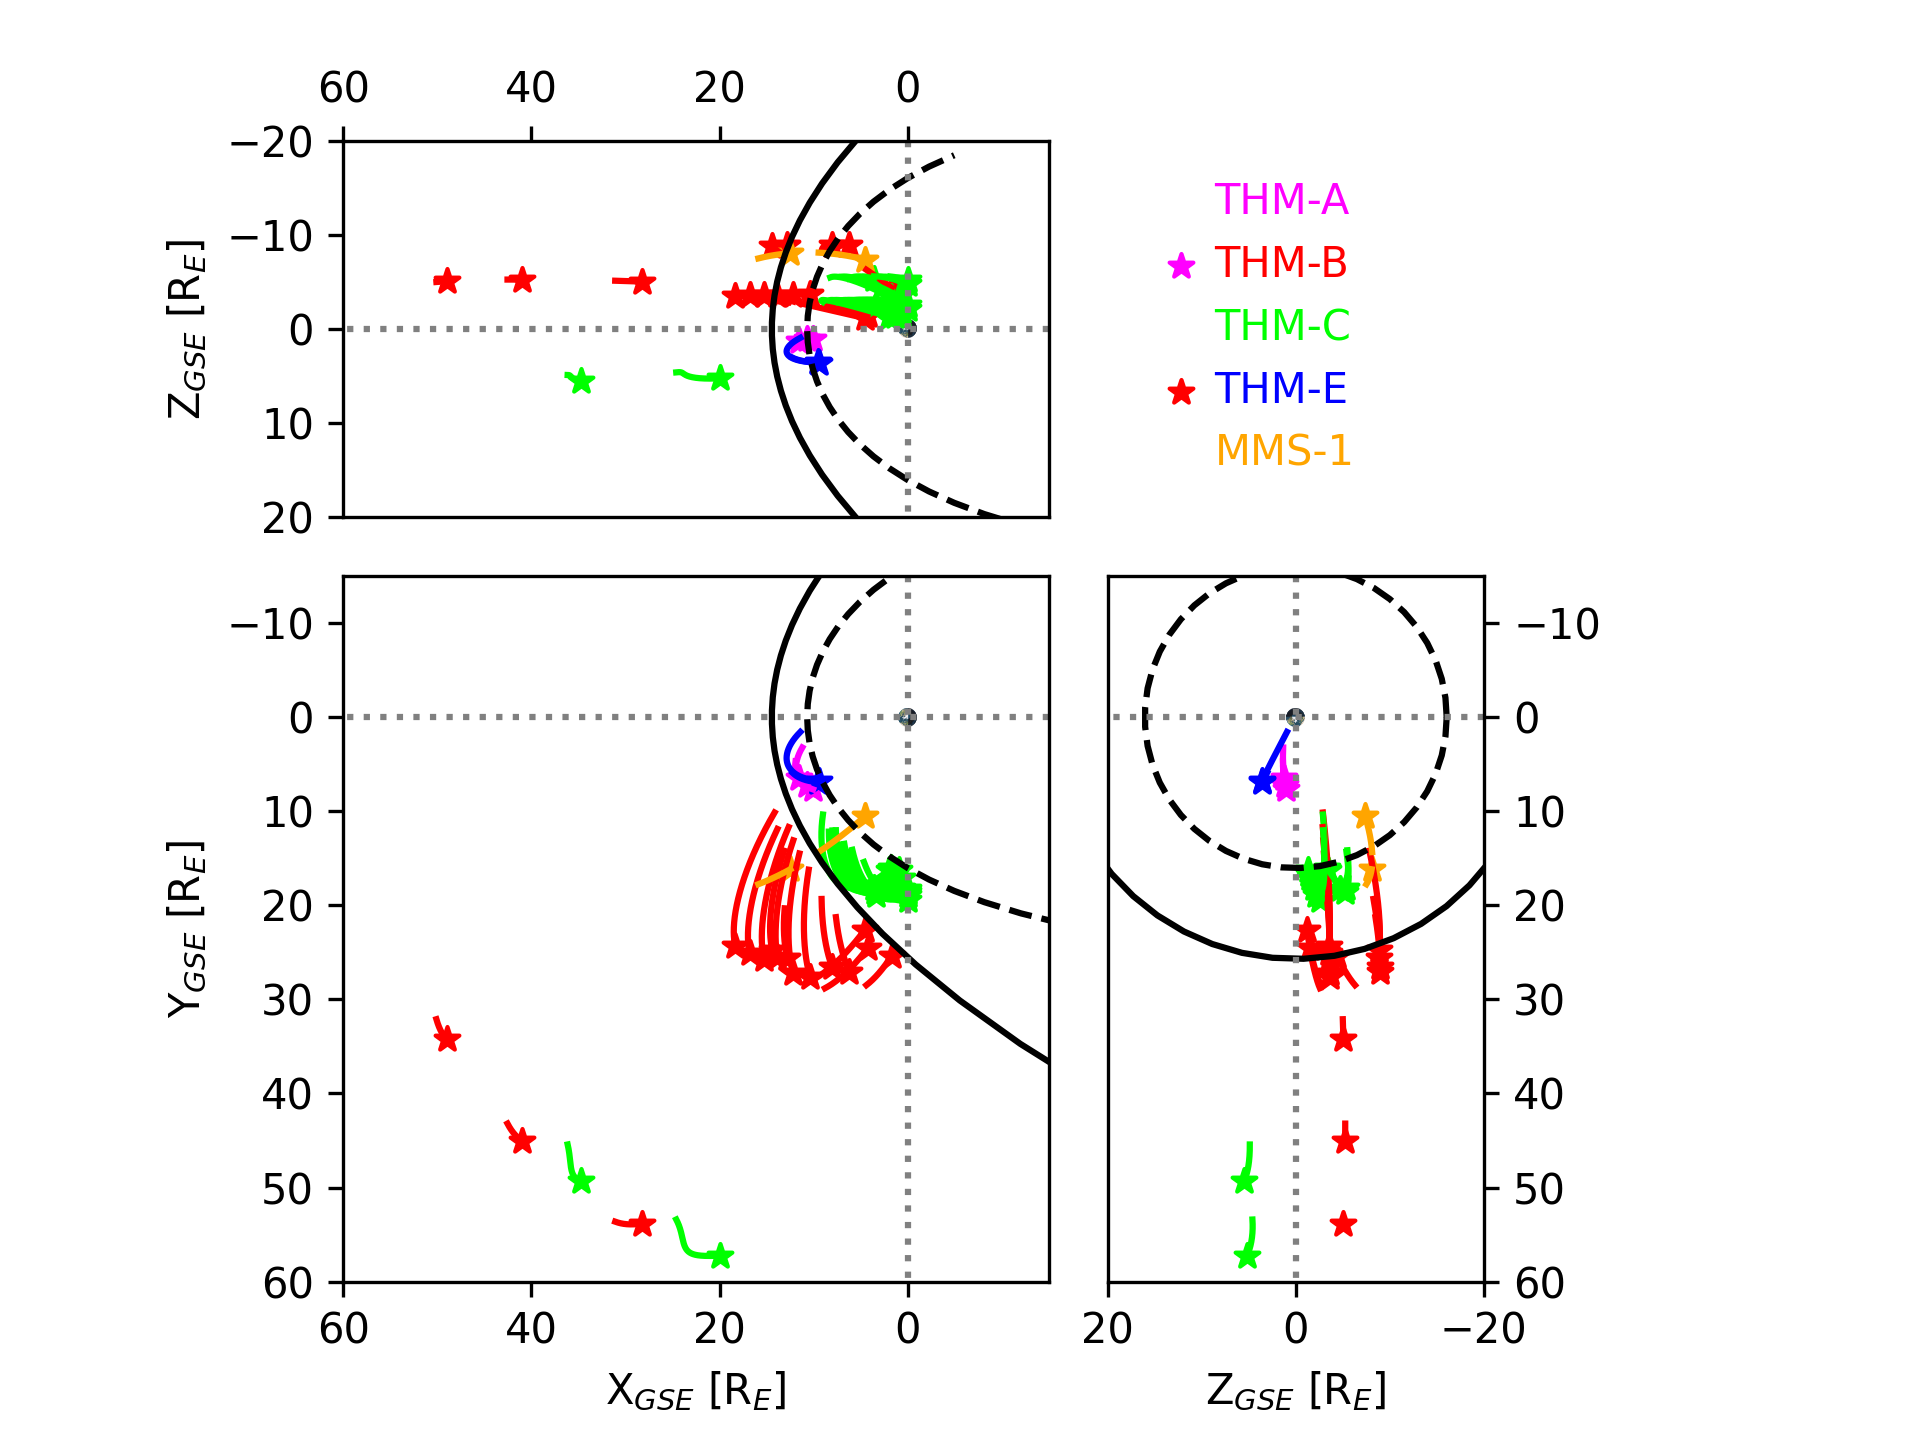
\includegraphics[width=\linewidth]{Figures/Orbits/all_TE_orbits_xy_xz_yz_coordinated.png}
    \caption[Orbits for coordinated analysis time periods]{Orbits for all time periods used in the coordinated study. Format follows that of Figure \ref{fig:orbits-all}.}
    \label{fig:orbits-coordinated}
\end{figure}


Figure \ref{fig:timeseries-THM-magnetosheath} is an example of one of the time periods observed in the magnetosheath during the coordinated analysis. These measurements were taken in the magnetosheath with THM-C, while the measurements in the solar wind were taken with THM-B. During the 19-20 June 2009 time period, THM-C experience a bow shock crossing, which is denoted by the grey-shaded interval in Figure \ref{fig:timeseries-THM-magnetosheath}. Periods of the identified intervals where bow shock crossings happened were removed from the resulting identified event lists. By looking at the time series data during the whole period, and identifying changes in the data such as magnetic field and ion spectra that were consistent with bow shock crossings \cite{Lalti:2022,Trotta:2022}, periods where the spacecraft were experiencing a bow shock crossing were identified. These bow shock crossing periods are removed so that chosen time periods are observed solely in one region per probe.

\begin{figure}
    \centering
    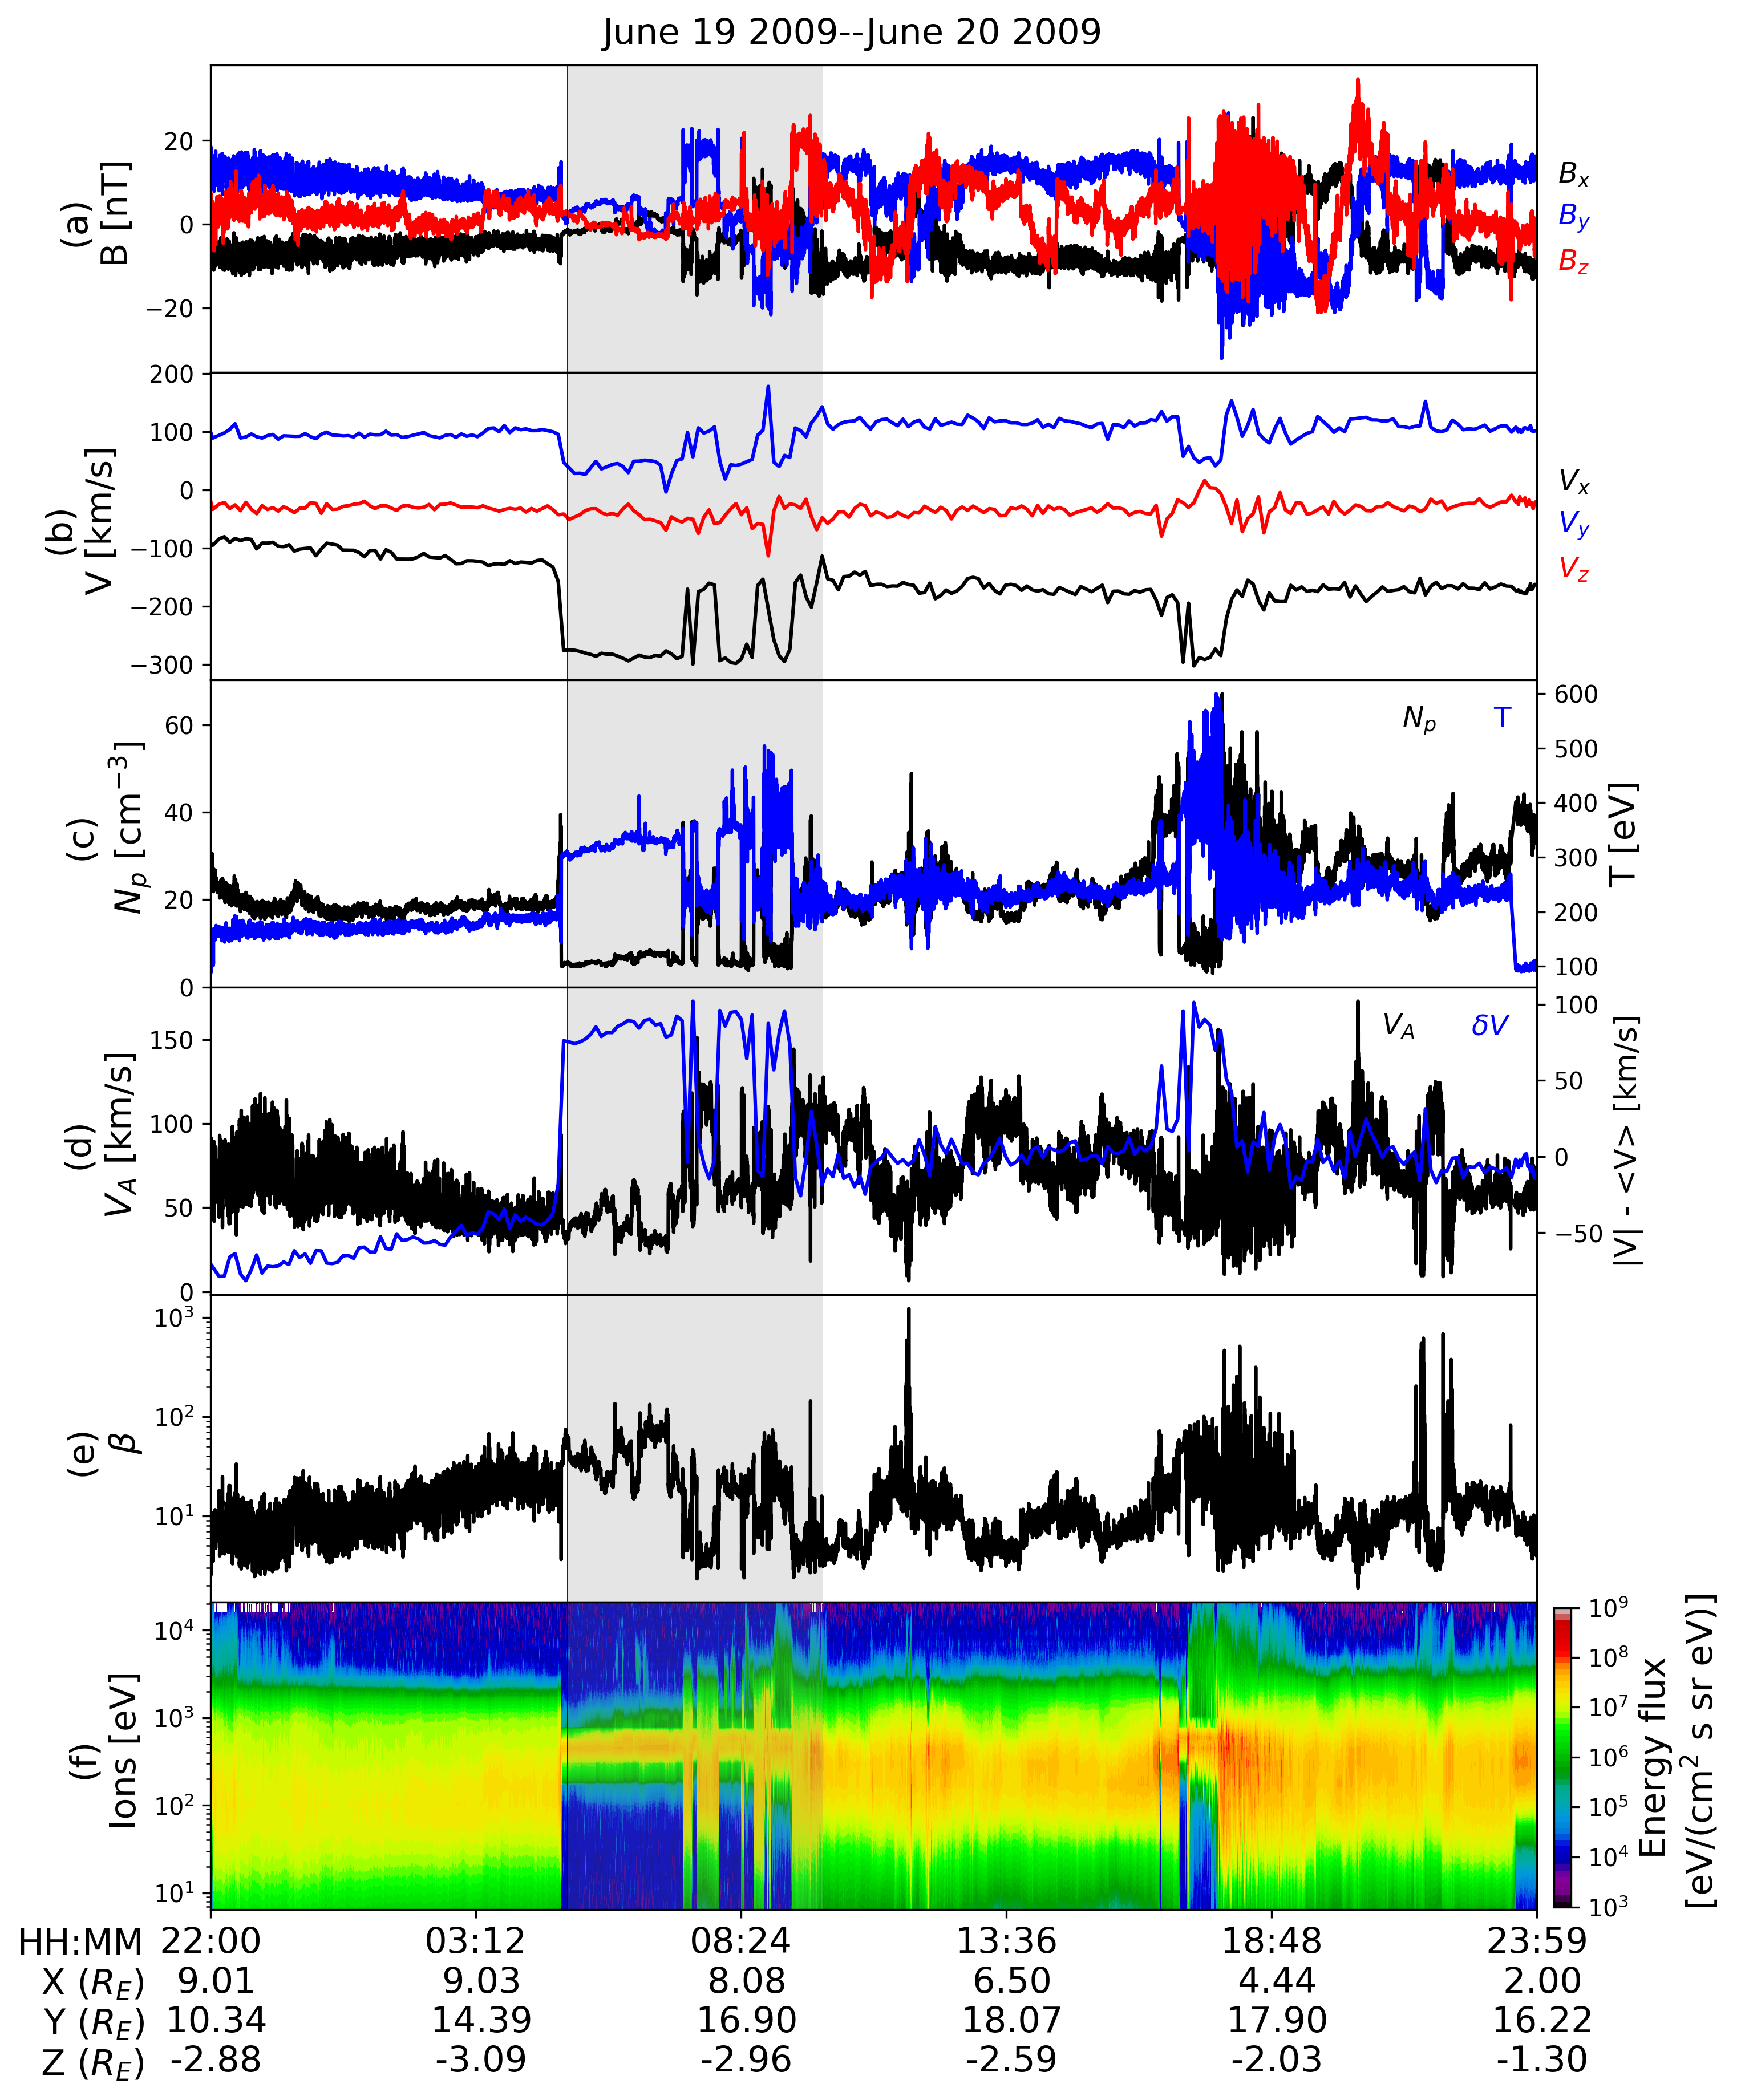
\includegraphics[width=\textwidth]{Figures/Time series/timeseries_19062009_THMC.png}
    \caption[Time series data for THM-C on 19-20 June 2009]{a) magnetic field, b) velocity, c) density and temperature, d) Alfv\'en speed and fluctuations of the magnitude of the velocity, e) plasma beta, and f) ion spectra for $\sim$26 hours in the magnetosheath on 19-20 June 2009. A bow shock crossing (grey region) is observed from 5:00-10:00 UT on 20 June 2009.}
    \label{fig:timeseries-THM-magnetosheath}
\end{figure}

\begin{figure}
    \centering
    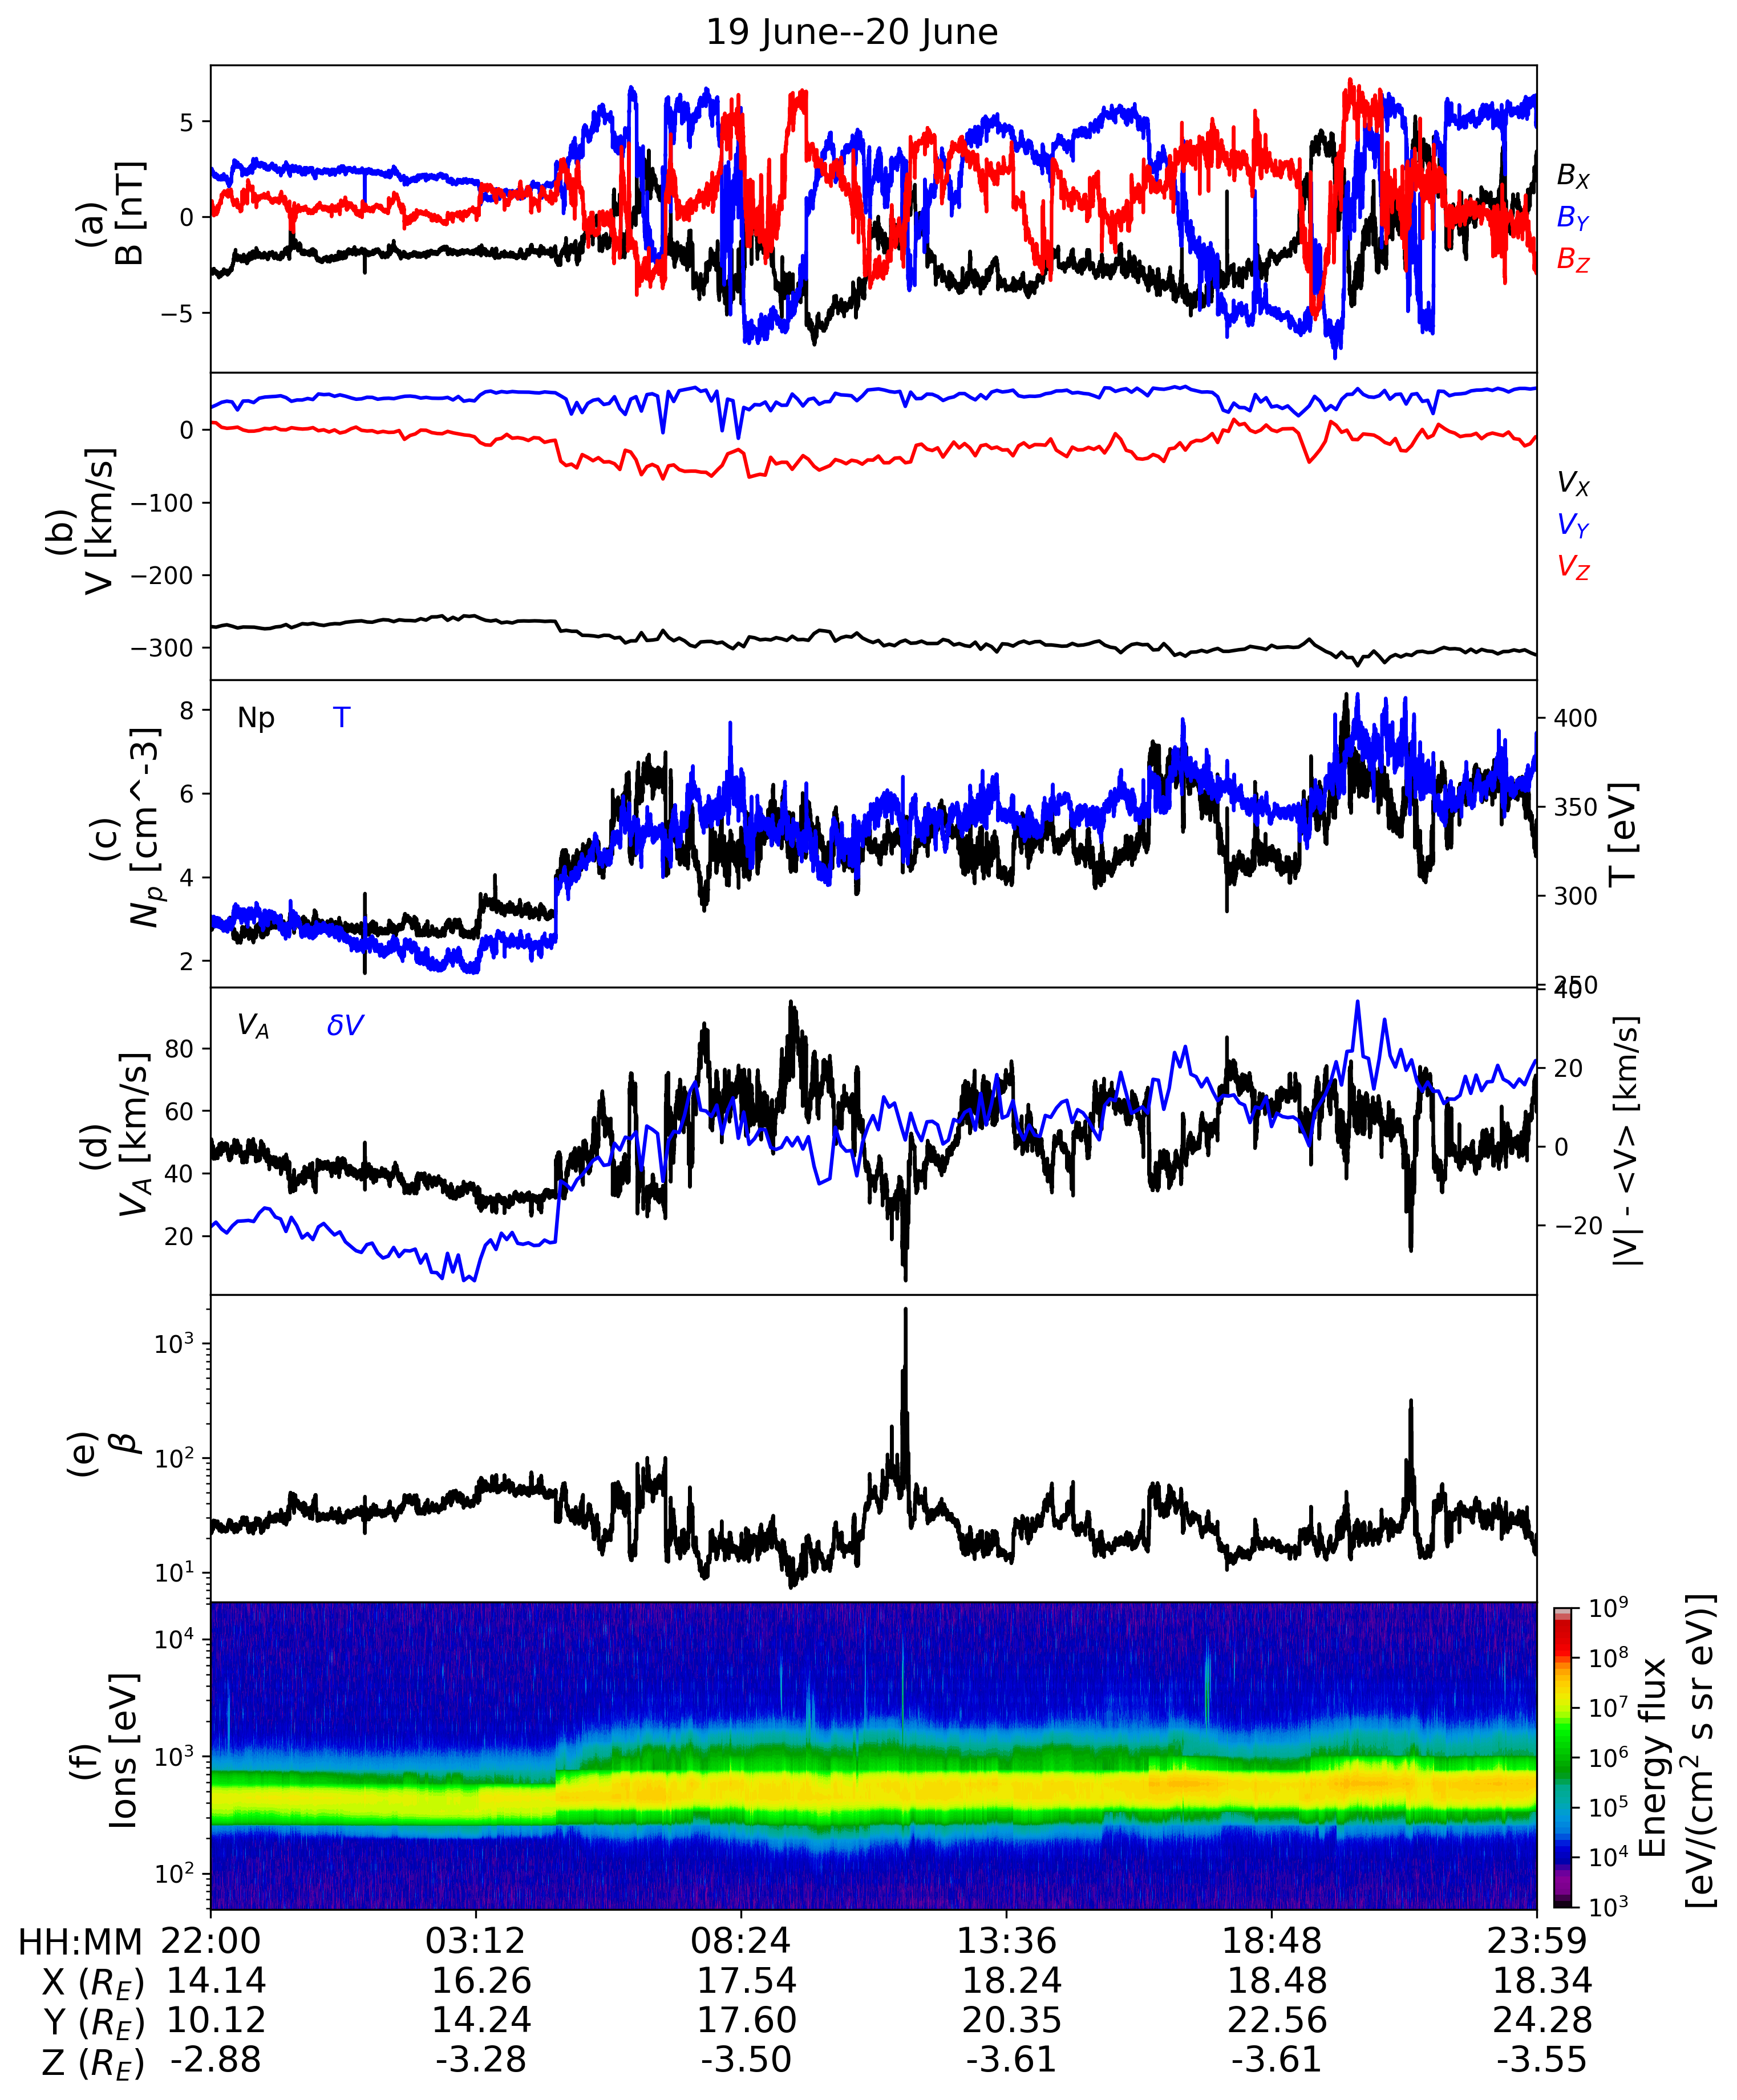
\includegraphics[width=\textwidth]{Figures/Time series/timeseries_19062009_THMB.png}
    \caption[Time series data for THM-B on 19-20 June 2009]{a) magnetic field, b) velocity, c) density and temperature, d) Alfv\'en speed and fluctuations of the magnitude of the velocity, e) plasma beta, and f) ion spectra for $\sim$26 hours in the solar wind (right) on 19-20 June 2009.}
    \label{fig:timeseries-THM-solarwind}
\end{figure}

% Toy-Edens list
In addition to identifying periods in solar wind and magnetosheath, the list of MMS data periods in the magnetosheath and solar wind from \cite{ToyEdens:2024} was also used. Their work focused on using unsupervised clustering to classify plasma regions in 8 years' worth of dayside MMS data. The 1-minute resolution data was classified into the regions: solar wind, ion foreshock, magnetosheath, and magnetosheath. The \cite{ToyEdens:2024} list contains over 9000 time periods in which MMS1-4 probes were identified to be solidly in the magnetosheath, with the minimum period being 15 minutes in length. 

The list \cite{ToyEdens:2024} was refined by taking time periods with a duration longer than 5 hours, which is comparable to the shortest identified time period of THEMIS data. 
%In order to ensure that the MMS probes were in the quasi-perpendicular region of the magnetosheath, only time periods in the list with $x_{GSE}>0\hspace{5pt}R_E$ and $y_{GSE}>0\hspace{5pt}R_E$. \citeA{ToyEdens2:2024} includes all MMS probes in their analysis; however, we only consider MMS-1 since presumably the other 3 MMS probes are in the same region. 107 time periods were obtained for this study from the Toy-Edens list 
After refining their magnetosheath list to the quasi-perpendicular magnetosheath, 107 time periods were obtained to be used in this study. 58 periods, in which MMS traversed the quasi-perpendicular solar wind, were obtained from the \cite{ToyEdens:2024} solar wind list. \cite{ToyEdens2:2024} includes all MMS probes in their analysis; however, we only consider MMS-1 since presumably the other 3 MMS probes are in the same region. In total, from the \cite{ToyEdens:2024} list and from our own identification, there were 130 time periods of data identified in the magnetosheath from THM-A, THM-C, THM-E, and MMS-1; and 77 periods identified in the solar wind from THM-B, THM-C, and MMS-1.

% note: 107 periods were used for detection; however of the total events, 5 events overlapped with mine that I had already run and then there was 1 period with data not available and 3 with time periods not really inside the magnetosheath by visual identification of time series data